\documentclass{beamer}

% NOTE: reference
% https://arxiv.org/pdf/1604.05488.pdf

% HAGAR, first telescope to operate at an elevation > 4km
% http://www.tifr.res.in/~hagar/
% https://en.wikipedia.org/wiki/Indian_Astronomical_Observatory


\mode<presentation> {\usetheme{Madrid}}

\usepackage{graphicx}
\usepackage[utf8]{inputenc}
\usepackage{amsmath, amsthm, amssymb, mathtools}
\usepackage{hyperref}
\usepackage{flexisym}
\usepackage{mhchem}
\usepackage{textcomp}
\usepackage[export]{adjustbox}
\usepackage{subfig}
\graphicspath{{./img/}}

\title[TeV Astrophysics]{Astronomical facilities and instrumentation in TeV}

\author{Wei-Chih Huang}
\institute[NTHU]{
National Tsing Hua University \\
\medskip
}
\date{April 23, 2019}


\begin{document}

\begin{frame}{ICAT: FACT}
	G-APD: a new semiconductor device with excellent single photon response became available: the so-called Geiger-mode Avalanche Photodiodes.
	\begin{figure}[h]
		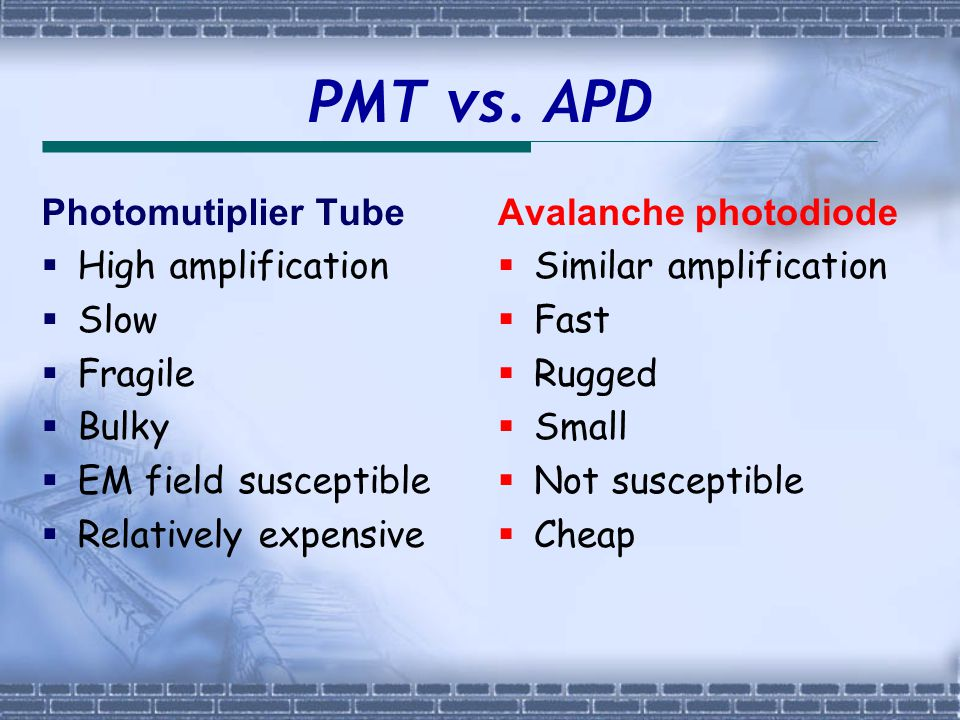
\includegraphics[width=280px]{PMTvsAPD.jpg}
	\end{figure}
\end{frame}


\begin{frame}{ICAT: FACT}
	\begin{figure}[h]
		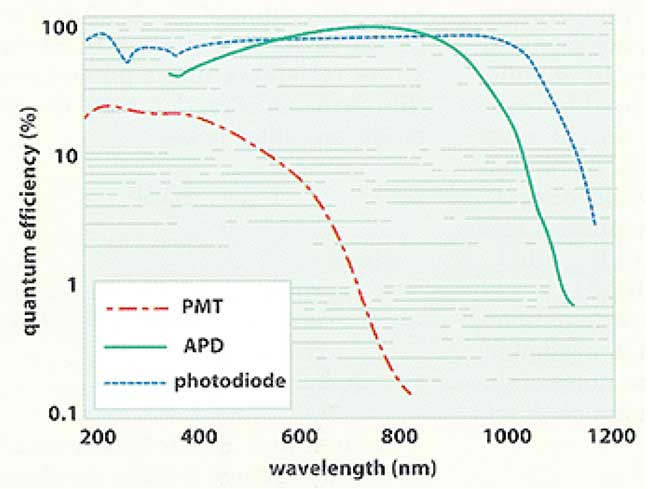
\includegraphics[width=280px]{DetectorsGuidepost.jpg}
	\end{figure}
\end{frame}

% \begin{frame}{ICAT: FACT}
% 	The Photomultiplier (PM) tube
% 	\begin{itemize}
% 		\item Detection of very weak scintillation light
% 		\item Provide electrical signal
% 		\item Can be also done with silicon photodiodes, but PM are most widely used
% 		\item Characterized by spectral sensitivity
% 	\end{itemize}
% \end{frame}


% \begin{frame}{ICAT: FACT}
	% Structure of PM tube
	% \begin{figure}[h]
		% 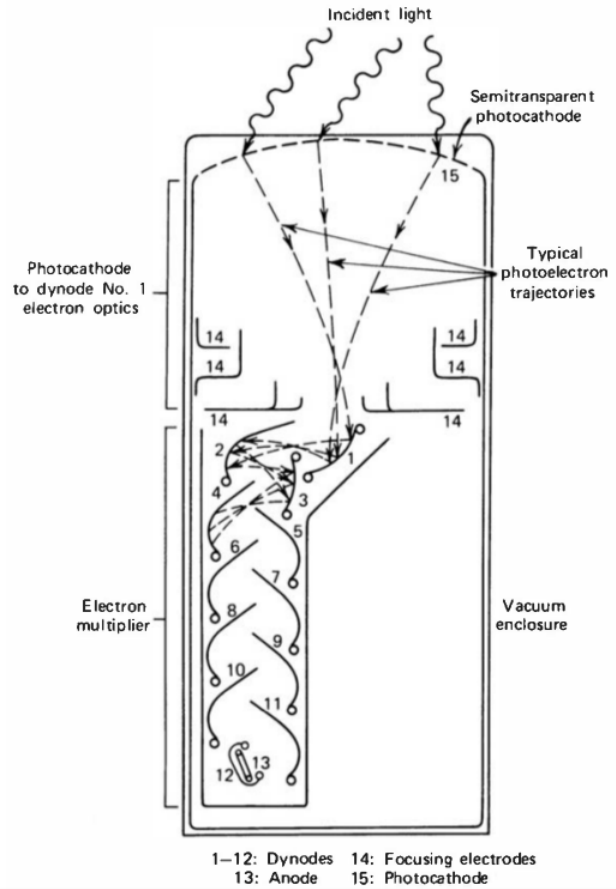
\includegraphics[width=280px]{PM_tube_structure.png}
	% \end{figure}
% \end{frame}


\begin{frame}{ICAT: FACT}
	First G-APD Cherenkov Telescope (FACT), which is based on a former HEGRA telescope.
	\newline
	\\
	Upgrade:
	\begin{itemize}
		\item refurbished mirrors
		\item drive system
	\end{itemize}
\end{frame}


\begin{frame}{ICAT: FACT}
	Mirrors:
	\begin{itemize}
		\item hexagonal shape surface with total area 9.51$m^2$
		\item re-machined by diamond-milling and subsequent coating with \ce{SiO2}.
	\end{itemize}
	\hfill \break
	Drive system:
	\begin{itemize}
		\item down-scaled version of the drive system implemented in the MAGIC telescopes
	\end{itemize}
\end{frame}

\begin{frame}{ICAT: FACT camera}
	\begin{itemize}
		\item 1440 pixels
		\item 4.5 degree FOV
		\item Photo sensors: G-APDs
		\item Solid light guides
	\end{itemize}
	\begin{figure}[h]
		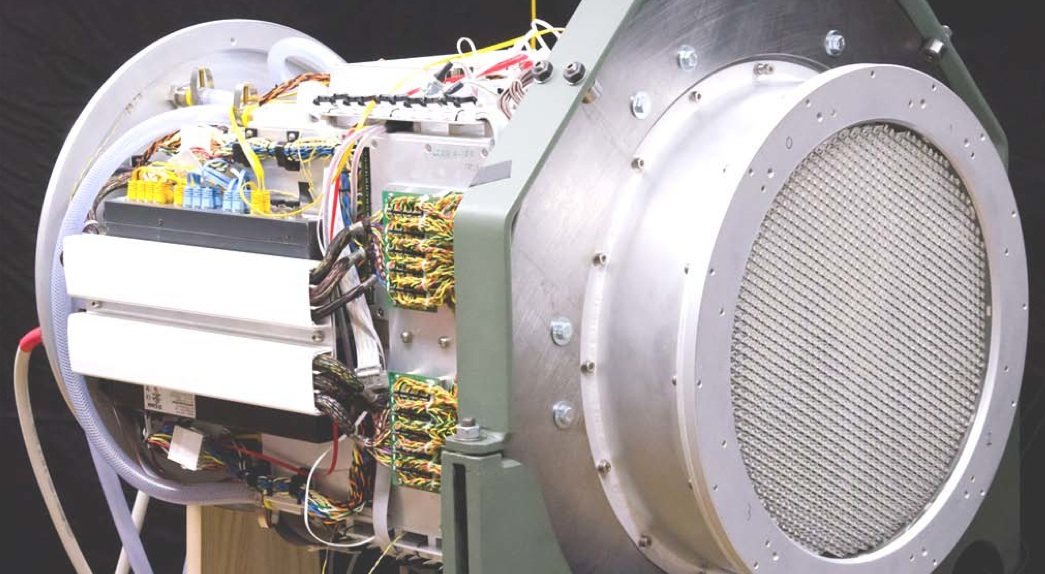
\includegraphics[width=280px]{ICATcamera.jpg}
	\end{figure}
\end{frame}



\begin{frame}{ICAT: FACT telescope}
	\begin{itemize}
		\item Location: 2200 m a.s.l., MAGIC site, Observatorio del Roque de los Muchachos, La Palma, Canary Islands, Spain
		\item Hexagonal mirrors
		\item Mirror area: 9.5 sqm
		\item Energy domain: TeV
	\end{itemize}
	\begin{figure}[h]
		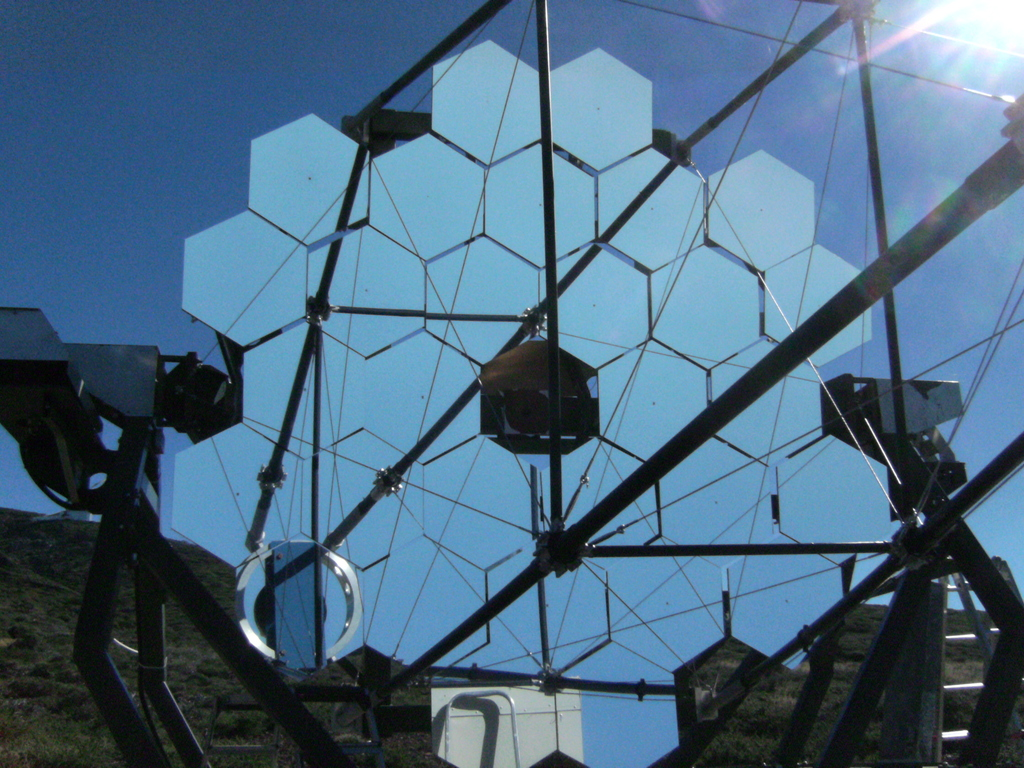
\includegraphics[width=200px]{FACTtelescope.jpg}
	\end{figure}
\end{frame}


\end{document}